\pagelayout{wide} % No margins
\myepigraphhead[500]{Should I kill myself or have a cup of coffee?}{Albert Camus}
\addpart{Introduction}
\pagelayout{margin} % Restore margins

\glsresetall % Reset glossary entries

\setchapterpreamble[u]{\margintoc}
\chapter{Context}
\labch{intro:context}

Technological development has undeniably improved material conditions for an
important part of humanity. Over the past century, innovations in energy,
medicine, transport, and communication have contributed to longer life
expectancy, higher productivity, and broader access to goods and services. This
has however been strongly correlated with major CO$_2$ emissions. For a time it
was at least possible to argue that this rise in emissions was tied to an
---unequal--- overall improvement in material well-being of \textit{some}
societies.

\begin{marginfigure}[-2.4cm]
    \includegraphics[]{shareholders-driven-apocalysis.png}
    \caption[Shareholders-driven apocalysis]{``Yes, the planet got destroyed.
    But for a beautiful moment in time, we created a lot of value for
    shareholders''\\Source:~\href{http://web.archive.org/web/20250808141700/https://www.newyorker.com/cartoon/a16995}{Tom
    Toro -- The New Yorker}}
    % \labfig{}
\end{marginfigure}

However, this trend has been reversed. Seven out of ten people live in
countries where economic inequality has increased over the past 30 years, and
nearly half of the world's wealth ---46~\%--- is concentrated in the hands of just
1~\% of the population~\sidecite[*6]{sayer_why_2016}.

We find ourselves in a paradoxical situation: as the planet becomes increasingly
uninhabitable, social inequalities continue to deepen. The overall outlook is
far from encouraging. Technological progress no longer serves to enhance
collective well-being\sidenote[][*3]{not that it ever did for a significant
amount of people~\cite{alcazar_rumbo_2023}} or to effectively build a
sustainable future. Instead, the relentless pursuit of endless economic growth
---fueled by unchecked consumption, short-term profit seeking, and a
shareholder-driven economy dominated by speculation--- is propelling us ever
closer to catastrophic climate collapse.

One of the main drivers in this direction, consequence of this unchecked growing
economy prioritization, is the  abuse in use of fossil fuels. Despite the finite
nature of fossil fuels, the problem today is not scarcity, but excess ---an
abundance sufficient to fill the atmosphere with greenhouse gases\sidenote{great
efforts are also being made in filling both hydrosphere and lithosphere with
plastics} at levels incompatible with life. The Paris Agreement has a long-term
temperature goal which is to keep the rise in global surface temperature to well
below 2~$^\circ$C above pre-industrial levels. The agreement also states that
preferably the limit of the increase should only be 1.5~$^\circ$C.

\begin{figure}
    \includegraphics[width=\textwidth]{global-mean-temperature-1850-2024.png}
    \caption{Annual global mean temperature anomalies relative to a
    pre-industrial (1850--1900) baseline. Source: State of the Global Climate.
    World Meteorological Organization
    (UN)~\cite{worldmeteorologicalorganization_state_2025}}
    \labfig{intro:global-mean-temperature}
\end{figure}

A 2024 report from the World Meteorological Organization (WMO) finds an 86~\%
chance that global average temperatures will exceed 1.5~$^\circ$C above
pre-industrial levels in at least one of the next five years (see
\reffig{intro:global-mean-temperature}), and a one per cent chance of one of
those years exceeding 2~$^\circ$C of
warming~\sidecite{worldmeteorologicalorganization_state_2025}.

Our dependence on fossil fuels is proving lethal, and this is manifesting in
multiple ways:

\begin{itemize}
    \item As of 2024, CO$_2$ emissions continue to increase, albeit more slowly
    than in the past. Yet this continued growth has pushed global emissions to
    another record high~\sidecite[*-4]{iea_global_2025}.
    
    \item Between 1999 and 2020, coal-related particulate matter (PM$_{2.5}$)
    caused an estimated 460,000 deaths in the United States
    alone~\sidecite[*-5]{henneman_mortality_2023}. 
    
    \item Plastic production has
    \href{https://ourworldindata.org/plastic-pollution?insight=plastic-production-has-more-than-doubled-in-the-last-two-decades}{more
    than doubled} in the last two decades~\sidecite{geyer_production_2017}. Only
    a small fraction of this plastic is recycled, and even then, only a limited
    number of times\sidenote{As environmental engineer
    \href{https://www.engineering.uga.edu/people/profile/jenna-jambeck-ph.d}{Jenna
    Jambeck} from the University of Georgia notes, ``What's the best way to
    manage waste? To not produce it in the first place.''}
    
    \item Studies covering nearly 750 extreme weather-related events and trends
    (see \reffig{intro:world-extreme-climate-events-map})
    show that 83~\% have been influenced by human-induced climate change~\cite{mcsweeney_mapped_2024}.
\end{itemize}

Even within this grim context, financial logic seems to prevail. Private
investors, motivated not by moral concern but by the growing profitability of
renewables, are now turning towards cleaner technologies\sidenote[][*-3]{The
private sector is driving the energy transition, providing three-quarters of
global clean energy investment. However, to meet scale investment in renewables
to at least USD$_{2025}$ 1.4 trillion per year in 2025--2030, more than doubling
the invested in 2024~\cite{irena_press_2025}}. Yet at the same time, a new wave
of governments has emerged that, despite overwhelming evidence, promotes a
return to fossil fuels: leaders who exploit crises to sow confusion and advance
regressive agendas\sidenote[][*-1]{Two examples:\\\textbf{·} President Trump
Prioritizes Fossil Fuel Development and Rolls Back Climate Action in
Energy~\cite{columbialawschool_president_2025}\\\textbf{·} Confusion over the
causes of the blackout intensifies the ideological battle between renewables and
nuclear power~\cite{eldiarioes_confusion_2025}}. If previous climate measures
were insufficient and often reduced to symbolic agreements with limited
implementation (\eg~Paris Agreement), the current political landscape shows an
even more concerning trend: \textit{open denialism}. This fuels widespread
disenchantment. Society has become increasingly alienated. Trust in collective
institutions, including science, is eroding, while conspiracy theories gain
traction and shape public opinion. As a result, genuine and complex challenges
are neglected, while artificial or symbolic issues dominate public discourse. In
Europe and elsewhere, racism and exclusionary politics are resurging, often
presented as responses to fabricated threats. Yet the true challenge lies ahead:
in the coming decades, climate change is expected to displace millions, as vast
regions of the planet become increasingly incompatible with human
life~\sidecite[*-5]{amelie_future_2025}.
% \textcolor{darkgray}{In Europe, despite targets such as recycling 55~\% of
% plastic packaging waste by 2030, most plastic waste was exported to China, where
% it ended up in landfills. In 2025, only around 12~\% is actually recycled. <--
% No sé de dónde saqué esto pero no es verdad, es el 40% }

\marginnote[]{
    \wideepigraph{State health services and pensions are run down and replaced by
    private health insurance and private pensions. You're on your own, free to
    choose, free to lose… Instead of seeing ourselves as members of a common
    society… we are supposed to see ourselves as competing individuals with no
    responsibility for anyone else.}{\textit{Andrew Sayer} \\ In \textit{Why We
    Can't Afford the Rich}}
}

\textbf{\textsc{The question}} remains whether societies will respond with
solidarity and structural transformation, or with further division and denial.


\section*{Where this research work fits in the current context}

After discussing the global environmental challenges of our time, and setting
aside their complex socio-political dimensions, the focus can now narrow to a
more specific and concrete contribution. The work presented here does not solve
such grand challenges, nowhere near, but rather contributes within a limited
scope: developing and optimizing technologies that improve the sustainable
management of two interconnected resources, energy and water, in two
solar-driven processes. A central element of this contribution is the
digitalization of these systems, enabling advanced modelling, prediction, and
optimization tools that are essential for improving the performance and
operational efficiency of solar-based technologies.


\begin{figure*}
    \includegraphics[width=\linewidth]{world-extreme-climate-events-map.png}
    \caption{Extreme weather-related events map. Source:~\cite{mcsweeney_mapped_2024}}
    \labfig{intro:world-extreme-climate-events-map}
\end{figure*}

This research is therefore structured in two complementary parts. The first
addresses the efficient management of water resources for power generation in
\gls{cspLabel} plants, through the optimization of a novel
combined cooling system. The second explores the efficient use of solar energy
for clean water production in a solar-driven multi-effect distillation system
with thermal storage, focusing once again on operational optimization.

In an era where almost every idea seems to have been expressed before,
originality rarely lies in invention alone, but in the creative integration
of existing concepts into meaningful, purposeful solutions. For this reason,
implementation plays an increasingly central role even ---and perhaps
especially--- in applied scientific research. Implementation should not remain
hidden; it should be shared, documented, and made accessible, allowing
others to replicate, verify, and build upon
it~\sidecite{hicks_bibliometrics_2015}.

Accordingly, the complete implementations of both studies are made available in
open repositories, alongside most of the code and supplementary material used to
develop this manuscript. The developed work has an important experimentation
component involving the facilities shown in \reffig{intro:pilot-plants}. Most
experimental and simulated results follow the \gls{fairLabel} data
principles\sidenote{And made public at time of publication of this manuscript.
The rest may follow soon after}~\sidecite{wilkinson_fair_2016}, ensuring
transparency, accessibility, and reproducibility. 

Further details are provided in \nrefsec{conclusions:contributions}.


\begin{figure}[htbp]
    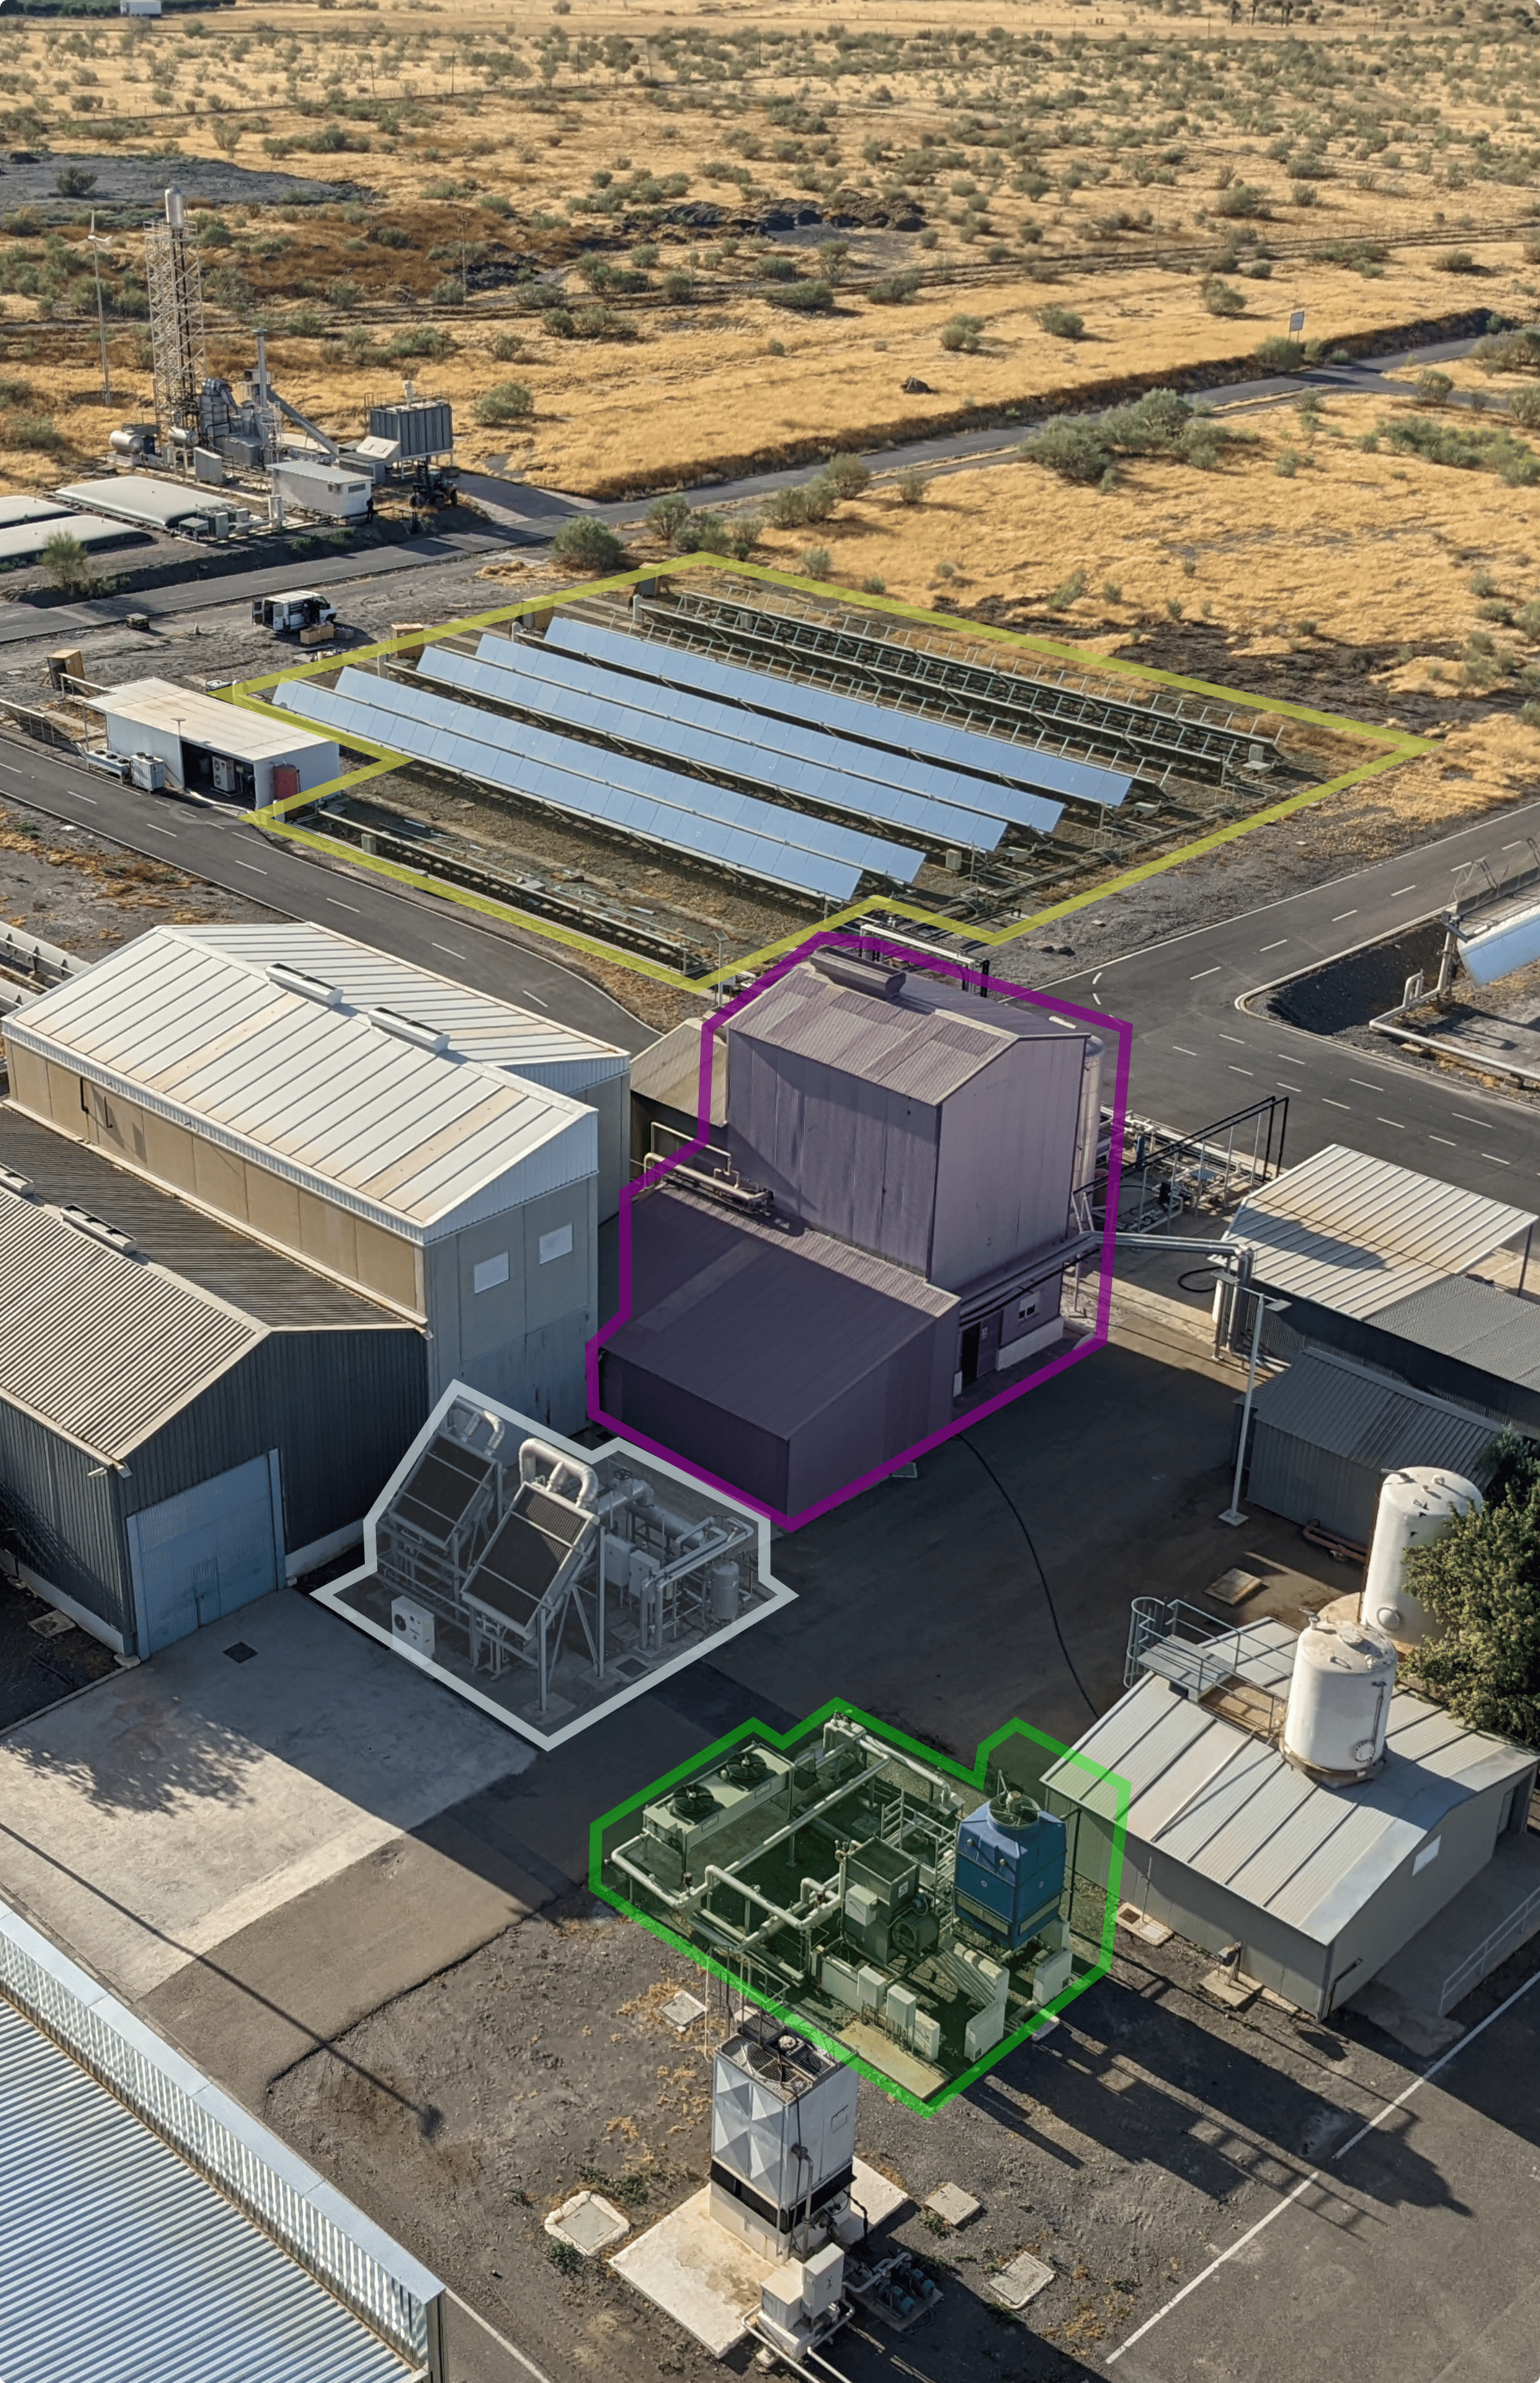
\includegraphics[width=\textwidth]{pilot-plants-aerial-view.png}
    \caption[Aerial view of the pilot plants at \gls{psaLabel}]{Aerial view
        of the pilot plants at \gls{psaLabel}, Spain.\\ 
        The developments presented in this thesis have
        been developed and validated around two test-rigs: a
        \gls{ccsLabel} and a \gls{solarmedLabel} pilot plant. In the picture,
        the solar field, the source of energy for all processes, is highlighted
        in yellow. Below it in purple is the building containing the
        \gls{medLabel} plant. The bottom two boxes (gray and green) delineate
        the area of the \gls{ccsLabel} plant. In gray the condenser and
        \gls{accLabel} and in green the combined cooler composed by the
        \gls{acheLabel} and \gls{wctLabel} components.
    }
    \labfig{intro:pilot-plants}
\end{figure}


%===================================
%===================================
%===================================
\setchapterpreamble[u]{\margintoc}
\chapter{Research plan}
\labch{intro:research-plan}


%===================================
%===================================
\section{Hypothesis}
\labsec{intro:research-plan:hypothesis}

The purpose of this thesis is to investigate the following hypotheses:

\begin{enumerate}[label=\roman*)]
    \item The selection of the cooling solution in a \gls{cspLabel} plant is
    strongly dependent on the specific location of the plant, particularly on
    its weather conditions and water resources. Restricting the cooling choice
    to only dry or only wet options penalizes the overall system performance.

    \item Hybrid or combined cooling systems are a technically feasible
    compromise between purely wet or dry systems, but they have seen limited
    deployment due to the increased complexity in design and operation. A
    general optimization methodology for these alternative cooling solutions
    could promote their broader adoption.

    \item Thermal desalination has an important role in addressing water
    scarcity, not necessarily as the dominant desalination technology, but by
    targeting specific applications where it can complement other mature
    processes. These include value-added approaches such as brine mining, as
    well as the recovery and treatment of industrial and mining wastewater
    streams where thermal methods offer clear advantages.

    \item To serve these niche but increasingly relevant applications, thermal
    desalination (with emphasis on \gls{medLabel}) must evolve in a sustainable and
    decarbonized direction. This requires, on the one hand, improving efficiency and
    expanding operational ranges, and on the other, adapting to low-temperature
    contexts where its heat demand can be met—partially or fully—using alternative
    sources such as low-exergy waste heat or solar thermal energy. While efficiency
    improvements are largely a design challenge, the present work contributes
    directly to the second aspect by developing methods that optimize the operation
    of solar-driven thermal desalination systems.
\end{enumerate}

%===================================
%===================================
\section{Objectives}
\labsec{intro:research-plan:objectives}

The specific objectives set out to fulfil in the present research work are
divided into two main blocks, each corresponding to one of the main
contributions of the thesis\sidenote{And matches the parts in this manuscript}.
The first block (\textbf{O1}) focuses on the development of a methodology for
the modelling and optimization of combined cooling systems, while the second
block (\textbf{O2}) is centered around \gls{medLabel} systems coupled with solar
thermal plants.

\begin{enumerate}[label=\textbf{O1.\arabic*}] 
    \item Model and validate various components of combined cooling systems, as
    well as their integration into a complete combined system.  
    \item Propose a methodology for optimizing combined cooling systems.  
    \item Experimental validation of the proposed methodology.  
    \item Perform a simulation-based analysis of a representative case study
    comparing different cooling alternatives and integrating the proposed
    methodology.
\end{enumerate}
\bigskip
\begin{enumerate}[label=\textbf{O2.\arabic*}]
    \item Analyze the current performance indices and evaluation criteria used
    in thermal desalination processes.  
    \item Establish a standardized experimental evaluation framework for thermal
    desalination processes using consistent performance criteria. 
    \item Design and assess basic control loops, as well as identify stable
    operating conditions to ensure the reliability of experimentally obtained
    evaluation criteria.  
    \item Experimentally evaluate improvements (\eg, nanofiltration
    pretreatment) that enhance efficiency and/or reduce costs in solar
    desalination systems.  
    \item Model and simulate multi-effect desalination plants coupled with solar
    thermal systems.  
    \item Propose a methodology to optimize the operation of solar desalination
    processes based on selected performance criteria.  
    \item Evaluate hierarchical control structures aimed at optimizing
    desalination processes coupled with solar plants.  
    \item Demonstrate that the proposed hierarchical control structures improve
    the performance indices of desalination plants coupled with solar thermal
    systems.  
\end{enumerate}

%===================================
%===================================
\section{Contributions}
\labsec{intro:research-plan:contributions}

Over the years, numerous studies have compared wet and dry cooling systems for
\gls{cspLabel} plants. Most of these works focus on sensitivity analyses of
selected operating
parameters~\sidecite{asfand_thermodynamic_2020,mdallal_modelling_2024,hu_thermodynamic_2018,
tang_study_2013,asvapoositkul_comparative_2014,barigozzi_performance_2014}. A
smaller number have addressed the optimization of individual component operation
to improve overall cooling system performance. In Martin \textit{et
al.}~\sidecite{martin_optimal_2013,martin_optimal_2015}, they optimized the
year-round operation of the cooling system (wet in~\cite{martin_optimal_2013}
and dry in~\cite{martin_optimal_2015}) in a \gls{cspLabel} plant. However, both of
their studies relied on monthly average data, which obscure significant daily
temperature variations ---often exceeding 10~$^\circ$C--- that coincide with
peak power production and substantially affect cooling system performance.

In contrast, there has been little discussion in the literature regarding the
operational strategies of combined cooling systems. For water-enhanced dry
cooling and parallel configurations, the commonly proposed
strategy~\sidecite{wiles_description_1978,zaloudek_study_1976,rohani_optimization_2021}
is to prioritize the dry section until the condenser pressure reaches a
predefined threshold, at which point the wet units are activated. While this
approach is simple and robust, it leaves significant performance potential
untapped.

Several additional considerations arise when developing an effective operation
strategy for combined cooling systems:
\begin{itemize}
    \item Humidity is typically higher at night, when ambient temperatures are
    lower. This partially mitigates the limitations of dry cooling and makes it
    less unfavorable.
    \item The wet cooling section should be fully leveraged when water is
    plentiful, given its superior efficiency and lower operational cost.
    \item The availability and dynamic cost of alternative water sources should
    be incorporated into the decision process.
    \item The operation of combined cooling systems is inherently complex and
    requires a strategy that, at a minimum, ensures reliable satisfaction of the
    cooling demand, and ideally, minimizes the total operating cost.
\end{itemize}

This research work investigates the optimization of different cooling system
configurations, focusing on their two main resource consumptions: electricity
and water. The optimization problems are formulated to minimize the total cost
of cooling a prescribed thermal load, with cost defined as the combined use of
these two resources. The thermal load itself is treated as an external
requirement and is therefore excluded from the decision space. This work
addresses existing gaps in the literature and, for the first time, presents an
actual optimization of the operation of a combined cooling system within the
context of \gls{cspLabel} applications.

\bigskip

Regarding the \gls{medLabel} process, its future in desalination and brine
concentration applications depends on both its technical development and its
integration with other
technologies~\sidecite[]{ghenai_performance_2021,son_pilot_2020}. Performance
evaluation plays a central role in this development. Although efforts have been
made to propose performance metrics for multi-effect evaporation, there is
currently neither consensus on which metrics are the most
appropriate~\sidecite{burgess_solar_2000} nor a standardized methodology for
experimental evaluation. The only existing standard for \gls{medLabel} processes
addresses cost structures and determinants rather than performance
assessment~\sidecite{pinto_desalination_2017}.

This research proposes a standardized methodology for evaluating the performance
of \gls{medLabel} processes, which can also be extended to other thermal
separation technologies. The method addresses key aspects such as
instrumentation requirements, process control, and the suitability of various
performance metrics, including the uncertainties associated with their
determination. In addition, an algorithm has been developed for the automatic
detection of steady-state operation, improving the reliability and robustness of
evaluations under variable conditions. Furthermore, the plant is evaluated for
the first time at high \glspl{tbtLabel} using the proposed methodology. The
results are analyzed using multiple performance metrics, and the scale formation
risk is quantified via the \gls{rsiLabel}.

\bigskip

A \gls{medLabel} plant, like any thermal separator, requires both heat and
electricity. While electricity costs can be directly assigned, the cost of
thermal energy depends on its source. When the heat is supplied by a variable
source such as solar (or waste) heat, the situation becomes more complex: solar
availability is intermittent, and the operation and efficiency of the solar
field are closely linked to how the \gls{medLabel} load is managed. This
coupling is further complicated by the presence of thermal storage, which allows
temporal shifting of heat usage and introduces additional operational decisions.

These promising low-exergy heat sources require high-level optimization systems
capable of managing fluctuating operating conditions in order to integrate them
with \gls{medLabel} processes. Most existing literature on the automatic control
of solar-driven \gls{medLabel} systems focuses on low-level control strategies,
typically employing simple control loops with either \gls{pidLabel}
controllers~\sidecite{roca_solar_2008a} or \gls{mpcLabel}
schemes~\sidecite{gonzalez_economic_2014a}, whose primary goal is to maintain
temperature setpoints ---usually at the heat source inlet. A number of works
have also addressed the optimization of the \gls{medLabel} process in
isolation~\sidecite{carballo_optimal_2018,chorak_experimental_2017}. However,
optimizing the \gls{medLabel} subsystem independently neglects its coupling with
the energy supply and storage systems.


Several studies have addressed this broader problem at varying levels of
complexity. González~\etal~\sidecite{gonzalez_economic_2014a} proposed
a receding-horizon optimal control strategy with economic objectives ---maximizing
water production while minimizing electricity costs--- but relied on a simplified
linear model that optimized only the solar field flow, keeping the
\gls{medLabel} inlet temperature constant. The most advanced optimization
efforts in the literature, however, have been developed for \gls{mdLabel}
rather than \gls{medLabel}. Gil~\etal~\sidecite{gil_hybrid_2019}
recognized that a solar \gls{mdLabel} plant operates through distinct modes
(\eg, solar field heating, thermal storage charging, and \gls{mdLabel}
operation), dictated by solar and thermal conditions. However, in their work,
the transitions between these modes were hardcoded in the control rules, meaning
that the choice of when to start or stop each subsystem was not treated as a
decision variable but as part of the environment.

In many studies, either the decision space is too limited, the models are overly
simplified, or key variables are treated as uncontrollable. Moreover, thermal
storage decouples heat usage from solar availability, within certain limits,
making the timing of subsystem operation ---both solar field and thermal
separator--- critical for maximizing system performance over multiple days. Using a
fixed irradiance threshold to trigger startup is therefore suboptimal, as it
ignores the state of thermal storage and forecasts of future solar availability,
which could enable more flexible and efficient operation.

In this work, the operation of a solar-driven \gls{medLabel} system is optimized
with these aspects explicitly accounted for. The formulation includes decision
variables for starting and stopping each subsystem and considers a two-day
prediction horizon. This enables the optimization to balance current
performance with the impact of present decisions on future operation. The method
is based on an experimentally validated system model that includes the
electrical consumption of each component, coupled with a comprehensive
data-driven \gls{medLabel} model.

\section{Implementation software tools}
\labsec{intro:tools}

Software development for this research relies on a variety of tools. Just as
scientific knowledge is built on the shoulders of giants\sidenote{Isaac Newton
in a letter to Robert Hooke in 1676, acknowledging that his discoveries were
built on the work of others; also the title of the fourth studio album by
English rock band Oasis}, software similarly builds upon thousands of ---mostly
open-source--- tools. Listing every tool used would be impractical, so only the most
relevant ones are presented below:

\begin{itemize}
    \item \href{https://github.com/esa/pygmo2}{PyGMO} (Mozilla Public License
    Version 2.0)~\sidecite{biscani_parallel_2020} is a Python library for
    massively parallel optimization. It provides a unified interface for
    optimization algorithms and problems, facilitating deployment in parallel
    environments.
    
    \item \href{https://github.com/SheffieldML/GPy}{GPy} (BSD-3-Clause License) 
    is a Gaussian Process Regression framework written in Python, developed by 
    the Sheffield Machine Learning group.
    
    \item \href{https://github.com/pytransitions/transitions}{pytransitions} 
    (MIT License) is a lightweight, object-oriented state machine implementation
    in Python with many extensions. Created by Tal Yarkoni and maintained by 
    Alexander Neumann.
    
    \item \href{https://github.com/m-lundberg/simple-pid}{simple-pid} (MIT License) 
    provides a simple and fast PID controller implementation in Python. Created 
    by Martin Lundberg.

    \item \href{https://github.com/apache/airflow}{Apache Airflow} (Apache 2.0
    License). A platform to programmatically author, schedule, and monitor
    workflows.

    \item \href{https://github.com/pyequion/pyequion2}{PyEquIon} (BSD 3-Clause
    License)~\sidecite{marcellos_pyequion_2021} is a Python package for
    automatic speciation calculations of aqueous electrolyte solutions.

    \item Statistics and Machine Learning Toolbox (proprietary MATLAB license) 
    provides functions and apps to describe, analyze, and model data, including 
    tools for machine learning such as classification, regression, clustering, 
    and dimensionality reduction.
\end{itemize}



